\documentclass[tikz,border=2pt]{standalone}
\usepackage{tikz,pgfplots,pgf}
\usetikzlibrary{decorations.pathmorphing,decorations.text,calc,snakes}
\newcommand{\MYPI}{3.14159}
\newcommand{\MYTHETA}{-20}
\newcommand{\MYSCALE}{3}
\newcommand{\XSHIFT}{0}
\newcommand{\OPRIME}{0}
\newcommand{\LINEPT}{3pt}
\DeclareMathSizes{20}{30}{20}{20}
\definecolor{myblue}{rgb}{0.0,0.447,0.741}
\definecolor{myblue2}{rgb}{0.301,0.745,0.933}
\definecolor{myorange}{rgb}{0.85,0.325,0.098}
\definecolor{mygreen}{rgb}{0.466,0.674,0.188}
\definecolor{mypurple}{rgb}{0.494,0.184,0.556}
\definecolor{myred}{rgb}{0.635,0.078,0.184}
\definecolor{myyellow}{rgb}{0.929,0.694,0.125}
\begin{document}
	\begin{tikzpicture}\label{fig:lattice1}
        \coordinate (Origin)   at (0,0);
    \coordinate (XAxisMin) at (0,0);
    \coordinate (XAxisMax) at (3,0);
    \coordinate (YAxisMin) at (0,0);
    \coordinate (YAxisMax) at (0,3);


    \draw[style=help lines,dashed,step=2] (0,0) grid (6,6);
    \foreach \x in {0,1,...,3}{% Two indices running over each
      \foreach \y in {0,1,...,3}{% node on the grid we have drawn
        \node[draw,circle,inner sep=2pt,fill, myblue](\x\y) at (2*\x,2*\y) {};
            % Places a dot at those points
      }
    }
    \draw [ myblue,-latex] (00) -- node[below] {$\textbf{a}_{1,0}$} (10);% Draw x axis
    \draw [ myblue,-latex] (00) -- node[left] {$\textbf{a}_{0,1}$} (01);% Draw y axis

    \end{tikzpicture}


    \begin{tikzpicture}\label{fig:lattice2}

    %\draw[style=help lines,dashed] (0,0) grid (3,3);
    \foreach \x in {0,1,...,3}{% Two indices running over each
      \foreach \y in {0,1,...,3}{% node on the grid we have drawn
        \node[draw,circle,inner sep=2pt,fill, mygreen](\x\y) at ({2*(cos(\MYTHETA)*\x + sin(\MYTHETA)*\y)},{2*(-sin(\MYTHETA)*\x + cos(\MYTHETA)*\y)}) {};
            % Places a dot at those points
      }
    }
    \draw [ mygreen,-latex] (00) -- node[below] {$\textbf{a}^{\prime}_{1,0}$} (10);% Draw x axis
    \draw [ mygreen,-latex] (00) -- node[left] {$\textbf{a}^{\prime}_{0,1}$} (01);% Draw y axis

    \foreach \x in {0,1,...,3}{% Two indices running over each
      \foreach \y [count=\yi] in {0,1,...,2}{% node on the grid we have drawn
        \draw [style=help lines,dashed] (\x\y) -- (\x\yi) (\y\x) -- (\yi\x);
            % Places a dot at those points
      }
    }


        \end{tikzpicture}

    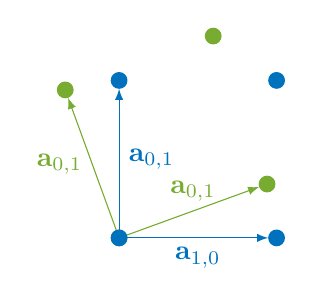
\begin{tikzpicture}\label{fig:latticecombined}

    %\draw[style=help lines,dashed] (0,0) grid (3,3);
    \foreach \x in {0,1,...,1}{% Two indices running over each
      \foreach \y in {0,1,...,1}{% node on the grid we have drawn
        \node[draw,circle,inner sep=2pt,fill, mygreen](l1\x\y) at ({2*(cos(\MYTHETA)*\x + sin(\MYTHETA)*\y)},{2*(-sin(\MYTHETA)*\x + cos(\MYTHETA)*\y)}) {};

        \node[draw,circle,inner sep=2pt,fill, myblue](l0\x\y) at (2*\x,2*\y) {};
            % Places a dot at those points
      }
    }

    \draw [ myblue,-latex] (l000) -- node[below] {$\textbf{a}_{1,0}$} (l010);
    \draw [ myblue,-latex] (l000) -- node[right] {$\textbf{a}_{0,1}$} (l001);

    \draw [ mygreen,-latex] (l100) -- node[left] {$\textbf{a}_{0,1}$} (l101);
    \draw [ mygreen,-latex] (l100) -- node[above] {$\textbf{a}_{0,1}$} (l110);

    \foreach \x in {0,1,...,3}{% Two indices running over each
      \foreach \y [count=\yi] in {0,1,...,2}{% node on the grid we have drawn
        %\draw [style=help lines,dashed] (l1\x\y) -- (l1\x\yi) (l1\y\x) -- (l1\yi\x);
        %\draw [style=help lines,dashed] (l0\x\y) -- (l0\x\yi) (l0\y\x) -- (l0\yi\x);


            % Places a dot at those points
      }
    }





    \end{tikzpicture}


\end{document}
